
% File acl2020.tex
%
%% Based on the style files for ACL 2020, which were
%% Based on the style files for ACL 2018, NAACL 2018/19, which were
%% Based on the style files for ACL-2015, with some improvements
%%  taken from the NAACL-2016 style
%% Based on the style files for ACL-2014, which were, in turn,
%% based on ACL-2013, ACL-2012, ACL-2011, ACL-2010, ACL-IJCNLP-2009,
%% EACL-2009, IJCNLP-2008...
%% Based on the style files for EACL 2006 by 
%%e.agirre@ehu.es or Sergi.Balari@uab.es
%% and that of ACL 08 by Joakim Nivre and Noah Smith

\documentclass[11pt,a4paper]{article}
\usepackage[hyperref]{acl2020}
\usepackage{times}
\usepackage{graphicx}
\usepackage{latexsym}
\usepackage{float}
\usepackage{placeins}
\usepackage{booktabs}
\renewcommand{\UrlFont}{\ttfamily\small}

% This is not strictly necessary, and may be commented out,
% but it will improve the layout of the manuscript,
% and will typically save some space.
\usepackage{microtype}

\aclfinalcopy % Uncomment this line for the final submission
%\def\aclpaperid{***} %  Enter the acl Paper ID here

%\setlength\titlebox{5cm}
% You can expand the titlebox if you need extra space
% to show all the authors. Please do not make the titlebox
% smaller than 5cm (the original size); we will check this
% in the camera-ready version and ask you to change it back.

\newcommand\BibTeX{B\textsc{ib}\TeX}

%%%%%%%%%%%%%%%%%%%%%%%%%%%%%%%%%%%%%%%%%%%%%%%%%%%%

\title{Hw1: Presidential Speech Classification with Word Embeddings}

\author{Sam Showalter \\
  University of California, Irvine \ (showalte) \\  
\texttt{showalte@uci.edu}} 

\date{}

%%%%%%%%%%%%%%%%%%%%%%%%%%%%%%%%%%%%%%%%%%%%%%%%%%%%

\begin{document}
\maketitle
\begin{abstract}
this is a testThis document contains the instructions for preparing a manuscript for the proceedings of ACL 2020.
The document itself conforms to its own specifications, and is therefore an example of what your manuscript should look like.
These instructions should be used for both papers submitted for review and for final versions of accepted papers.
Authors are asked to conform to all the directions reported in this document.
\end{abstract}


%%%%%%%%%%%%%%%%%%%%%%%%%%%%%%%%%%%%%%%%%%%%%%%%%%%%
% Introduction
%%%%%%%%%%%%%%%%%%%%%%%%%%%%%%%%%%%%%%%%%%%%%%%%%%%%
\section{Introduction}










%%%%%%%%%%%%%%%%%%%%%%%%%%%%%%%%%%%%%%%%%%%%%%%%%%%%
% Supervised Learning Grid Search
%%%%%%%%%%%%%%%%%%%%%%%%%%%%%%%%%%%%%%%%%%%%%%%%%%%%
\section{Supervised Learning}%
\label{sec:supervised_learning}




%%%%%%%%%%%%%%%%%%%%%%%%%%%%%%%%%%%%%%%%%%%%%%%%%%%%
% Feature Engineering
%%%%%%%%%%%%%%%%%%%%%%%%%%%%%%%%%%%%%%%%%%%%%%%%%%%
\subsection{Feature Engineering}%
\label{sub:feature_engineering}
%%%%%%%%%%%%%%%%%%%%%%%%%%%%%%%%%%%%%%%%%%%%%%%%%%%%


%%%%%%%%%%%%%%%%%%%%%%%%%%%%%%%%%%%%%%%%%%%%%%%%%%%%
% Stopwords token filtering figure
%%%%%%%%%%%%%%%%%%%%%%%%%%%%%%%%%%%%%%%%%%%%%%%%%%%%
\begin{figure}[htpb]
  \centering
  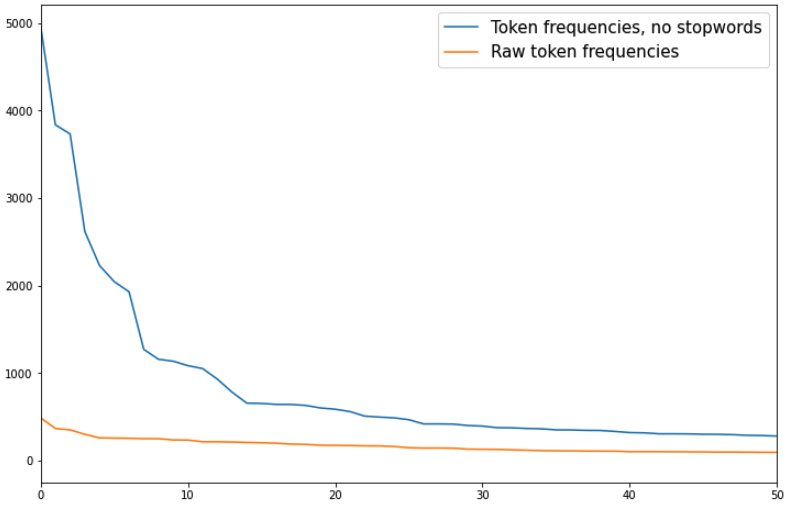
\includegraphics[width=1\linewidth]{imgs/stopwords.png}
  \caption{Token frequencies in training data before and after 
  stopwords removed from the dataset}%
  \label{fig:stopwords}
\end{figure}
%%%%%%%%%%%%%%%%%%%%%%%%%%%%%%%%%%%%%%%%%%%%%%%%%%%%

%%%%%%%%%%%%%%%%%%%%%%%%%%%%%%%%%%%%%%%%%%%%%%%%%%%%
% Token dimensionality exploration
%%%%%%%%%%%%%%%%%%%%%%%%%%%%%%%%%%%%%%%%%%%%%%%%%%%%
\begin{figure}[htpb]
  \centering
  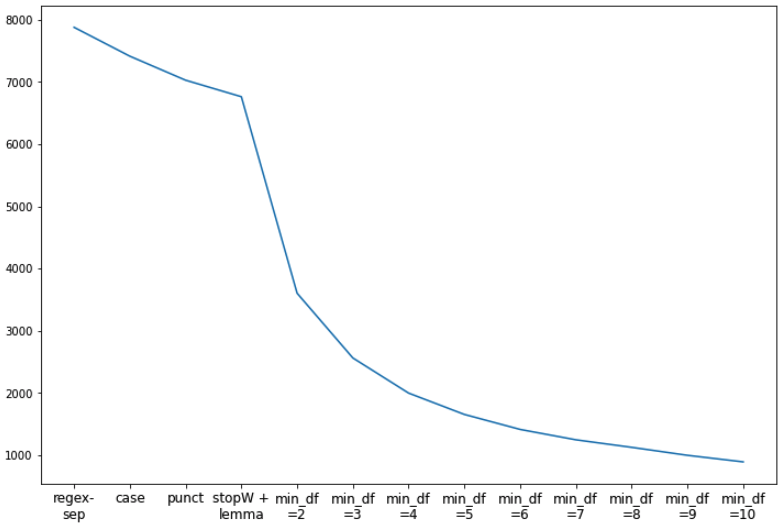
\includegraphics[width=1\linewidth]{imgs/token_filter.png}
  \caption{Vocabulary size as successive filters applied to input corpus. 
    From left to right, the strings are regex separated, then case and
  punctuation is resolved, with final filters trimming rare tokens}
  \label{fig:imgs/token_filter}
\end{figure}
%%%%%%%%%%%%%%%%%%%%%%%%%%%%%%%%%%%%%%%%%%%%%%%%%%%%



%%%%%%%%%%%%%%%%%%%%%%%%%%%%%%%%%%%%%%%%%%%%%%%%%%%%
% Feature engineering grid search table
%%%%%%%%%%%%%%%%%%%%%%%%%%%%%%%%%%%%%%%%%%%%%%%%%%%%
\FloatBarrier
\begin{table}[h]
    \centering
    \caption{Feature Engineering Grid Search}
    \begin{tabular}{
    	l
        l
        l
        l
        l
        l
        }
        \toprule
        \multicolumn{2}{c}{} &
        \multicolumn{4}{c}{Language Feature Filters}\\
        \cmidrule(lr){3-6} 
        {Token}& {Tok.} &{None} &{Case+}&{Lem.}& {Stop}\\
        {Engine} & {Sep.} && {Punct.}&&{Word}\\
        \midrule
      CVect & nltk & 0.399& \textbf{0.435}& \textbf{0.435}& 0.401\\
        CVect & reg& 0.396& 0.413&0.413& 0.399\\
        Tf-Idf & nltk & 0.382&  0.382 &0.382 & 0.386\\
        Tf-Idf & reg & 0.360& 0.374 & 0.374& 0.381\\
        \bottomrule
    \end{tabular}
\end{table}
\FloatBarrier
%%%%%%%%%%%%%%%%%%%%%%%%%%%%%%%%%%%%%%%%%%%%%%%%%%%%


%%%%%%%%%%%%%%%%%%%%%%%%%%%%%%%%%%%%%%%%%%%%%%%%%%%%
% Dimensionality Reduction
%%%%%%%%%%%%%%%%%%%%%%%%%%%%%%%%%%%%%%%%%%%%%%%%%%%%
\subsection{Dimensionality Reduction}%
\label{sub:dimensionality_reduction}
%%%%%%%%%%%%%%%%%%%%%%%%%%%%%%%%%%%%%%%%%%%%%%%%%%%%

this should word \cite{pennington2014glove} this should word

%%%%%%%%%%%%%%%%%%%%%%%%%%%%%%%%%%%%%%%%%%%%%%%%%%%%
% Dimensionality Rediction Figure
%%%%%%%%%%%%%%%%%%%%%%%%%%%%%%%%%%%%%%%%%%%%%%%%%%%%
\begin{figure}[htpb]
  \centering
  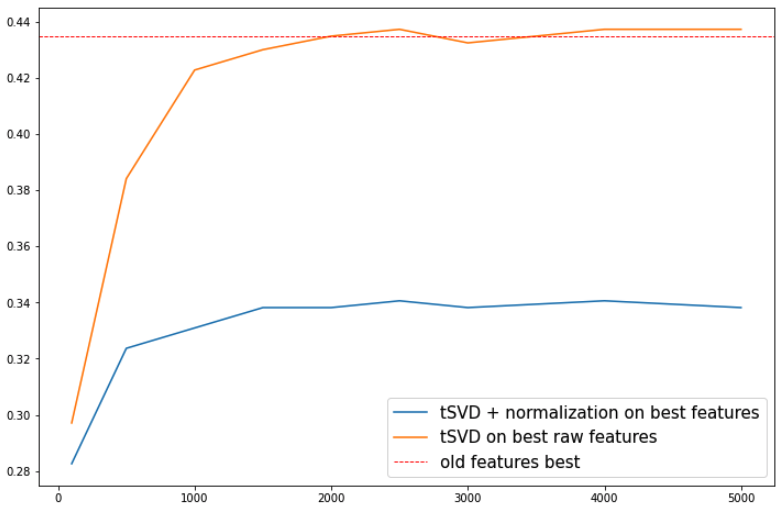
\includegraphics[width=1\linewidth]{imgs/tsvd.png}
  \caption{Classification performance applied to best feature
  selection after Truncated SVD applied with varying numbers of 
 components}%
  \label{fig:tsvd}
\end{figure}
%%%%%%%%%%%%%%%%%%%%%%%%%%%%%%%%%%%%%%%%%%%%%%%%%%%%



%%%%%%%%%%%%%%%%%%%%%%%%%%%%%%%%%%%%%%%%%%%%%%%%%%%%
% Model Ablation
%%%%%%%%%%%%%%%%%%%%%%%%%%%%%%%%%%%%%%%%%%%%%%%%%%%
\subsection{Model Tuning}%
\label{sub:model_tuning}

%%%%%%%%%%%%%%%%%%%%%%%%%%%%%%%%%%%%%%%%%%%%%%%%%%%%


%%%%%%%%%%%%%%%%%%%%%%%%%%%%%%%%%%%%%%%%%%%%%%%%%%%%
% Model Grid Search Plot
%%%%%%%%%%%%%%%%%%%%%%%%%%%%%%%%%%%%%%%%%%%%%%%%%%%%
\begin{table}[h]
    \centering
    \caption{Model Tuning: Logistic Regression}
    \begin{tabular}{
    	l
        l
        l
        l
        l
        l
        }
        \toprule
        \multicolumn{1}{c}{} &
        \multicolumn{5}{c}{Logistic Reg. Solver}\\
        \cmidrule(lr){2-6} 
        {Reg.}& {lbfgs} &{lib-} &{newton}&{saga}& {sag}\\
        {Pen.} & {} &{linear}& {}&&{}\\
        \midrule
        - & 0.399 & - & 0.401 & \textbf{0.454} & 0.447\\
        L1 & - & 0.423 &  -&0.428& -\\
        L2 & 0.447& 0.432& 0.450& 0.447& \textbf{0.450}\\
        \bottomrule
    \end{tabular}
\end{table}
%%%%%%%%%%%%%%%%%%%%%%%%%%%%%%%%%%%%%%%%%%%%%%%%%%%%


%%%%%%%%%%%%%%%%%%%%%%%%%%%%%%%%%%%%%%%%%%%%%%%%%%%%
% Semi-Supervised Learning
%%%%%%%%%%%%%%%%%%%%%%%%%%%%%%%%%%%%%%%%%%%%%%%%%%%%
\section{Semi-supervised Learning with Word Embeddings}%
\label{sec:semi_supervised_learning_with_word_embeddings}


%%%%%%%%%%%%%%%%%%%%%%%%%%%%%%%%%%%%%%%%%%%%%%%%%%%%
% Word2Vec
%%%%%%%%%%%%%%%%%%%%%%%%%%%%%%%%%%%%%%%%%%%%%%%%%%%%
\subsection{Word2Vec for Text Classification}%
\label{sub:word2vec_for_text_classification}

%%%%%%%%%%%%%%%%%%%%%%%%%%%%%%%%%%%%%%%%%%%%%%%%%%%%
% Word2Vec PCA example
%%%%%%%%%%%%%%%%%%%%%%%%%%%%%%%%%%%%%%%%%%%%%%%%%%%%
\begin{figure}[htpb]
  \centering
  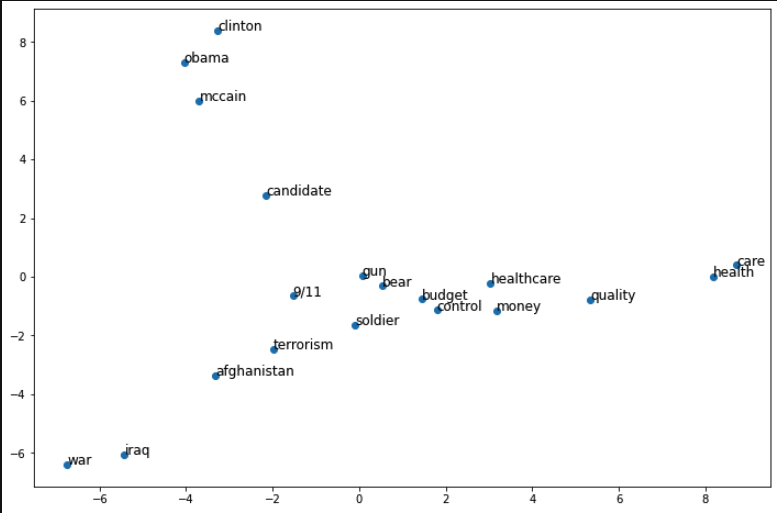
\includegraphics[width=1\linewidth]{imgs/w2v_pca.png}
  \caption{Visualization of Word2Vec embeddings with PCA with a selection 
  of common political terms. Embeddings appear to capture some level of 
semantic meaning}%
  \label{fig:imgs/w2v_pca}
\end{figure}

%%%%%%%%%%%%%%%%%%%%%%%%%%%%%%%%%%%%%%%%%%%%%%%%%%%%






%%%%%%%%%%%%%%%%%%%%%%%%%%%%%%%%%%%%%%%%%%%%%%%%%%%%
% Results and Discussion
%%%%%%%%%%%%%%%%%%%%%%%%%%%%%%%%%%%%%%%%%%%%%%%%%%%%

\section{Experimental Results and Discussion}%
\label{sec:experimental_results_and_discussion}


%%%%%%%%%%%%%%%%%%%%%%%%%%%%%%%%%%%%%%%%%%%%%%%%%%%%
% Word2Vec Performance
%%%%%%%%%%%%%%%%%%%%%%%%%%%%%%%%%%%%%%%%%%%%%%%%%%%%
\begin{figure}[htpb]
  \centering
  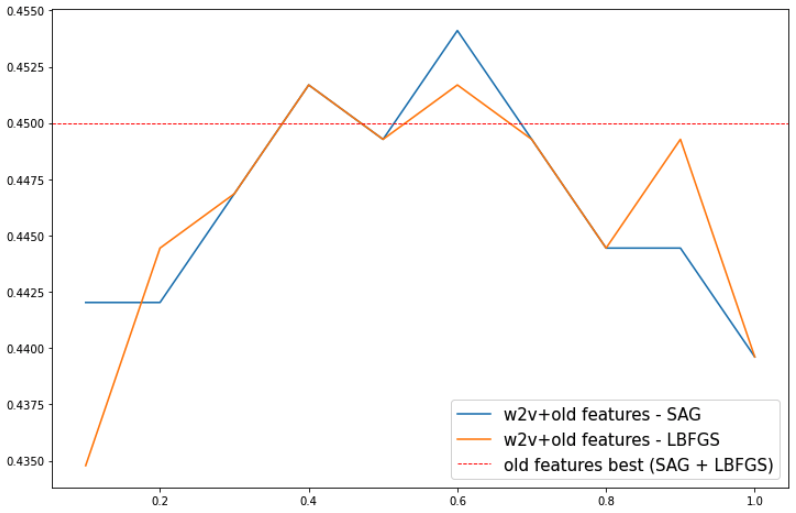
\includegraphics[width=1\linewidth]{imgs/w2v_classification.png}
  \caption{Classification performance of Word2Vec document embeddings with
  and without original SVD features concatenated. The x-axis represents
the fraction of unlabeled documents leveraged to make the Word2Vec model}%
  \label{fig:imgs/w2v_classification}
\end{figure}

%%%%%%%%%%%%%%%%%%%%%%%%%%%%%%%%%%%%%%%%%%%%%%%%%%%%


%%%%%%%%%%%%%%%%%%%%%%%%%%%%%%%%%%%%%%%%%%%%%%%%%%%%
% Word2Vec Candidate Embeddings
%%%%%%%%%%%%%%%%%%%%%%%%%%%%%%%%%%%%%%%%%%%%%%%%%%%%
\begin{figure}[htpb]
  \centering
  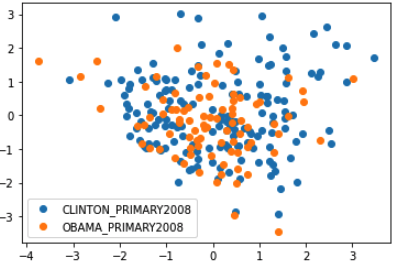
\includegraphics[width=1\linewidth]{imgs/PCA_w2v_Obama.png}
  \caption{Visualization of political candidate embedding profiles
  as defined by their speech embeddings. Little separation can be cleaned,
likely because order is not considered in embedding creation}%
  \label{fig:imgs/PCA_w2v_Obama}
\end{figure}
%%%%%%%%%%%%%%%%%%%%%%%%%%%%%%%%%%%%%%%%%%%%%%%%%%%%



%%%%%%%%%%%%%%%%%%%%%%%%%%%%%%%%%%%%%%%%%%%%%%%%%%%%
% Conclusion
%%%%%%%%%%%%%%%%%%%%%%%%%%%%%%%%%%%%%%%%%%%%%%%%%%%%
\section{Conclusions and Further Exploration}%
\label{sec:conclusion_and_further_exploration}

%%%%%%%%%%%%%%%%%%%%%%%%%%%%%%%%%%%%%%%%%%%%%%%%%%%%


\bibliography{custom}
\bibliographystyle{acl_natbib}

\appendix


\section{Statement of Collaboration}

\end{document}% File acl2020.tex

